\documentclass[tikz]{standalone}
\usepackage{pgfplots}
\pgfplotsset{compat=1.15}
\usepackage{mathrsfs}
\usetikzlibrary{arrows,calc}
\usepackage{tkz-euclide}
\pagestyle{empty}

\definecolor{AngleClr}{rgb}{0,0.39215686274509803,0}
\definecolor{ShapeClr}{rgb}{0.6,0.2,0}
\definecolor{BlueClr}{RGB}{13,93,184}

\begin{document}

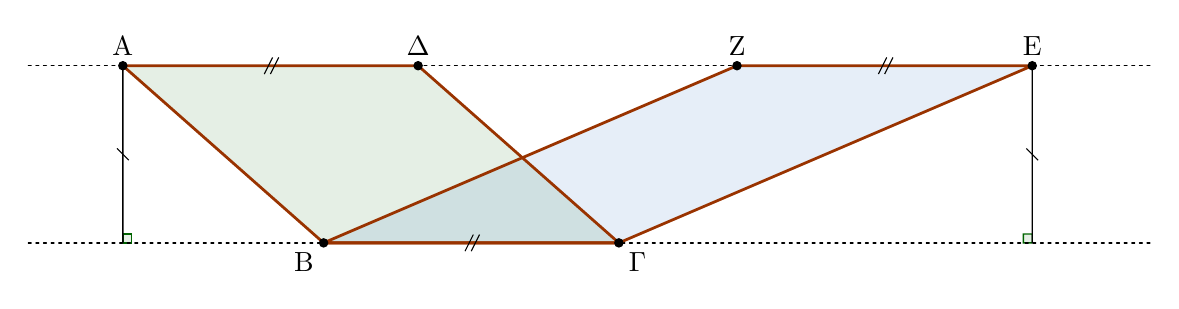
\begin{tikzpicture}[scale=.75]
\tkzSetUpLine[line width=1pt,color=black]
\tkzSetUpPoint[fill=black]

\tkzDefPoints{0/0/B,-3.4/3/A,5/0/C,1.6/3/D,7/3/Z,12/3/E}

\tkzDefPoints{-5/3/L1,14/3/R1}
\tkzDefPoints{-5/0/L2,14/0/R2}

\tkzDefPointBy[projection=onto B--C](A)\tkzGetPoint{AA}
\tkzDefPointBy[projection=onto B--C](E)\tkzGetPoint{EE}
\tkzMarkRightAngles[line width=0.5pt, size=.15,color=AngleClr,fill=AngleClr,fill opacity=0.1](A,AA,B E,EE,C)


\tkzFillPolygon[fill=AngleClr,fill opacity=0.1](A,B,C,D)
\tkzFillPolygon[fill=BlueClr,fill opacity=0.1](B,C,E,Z)


\tkzDrawSegments[line width=0.5pt,color=black,dashed,dash pattern=on 1pt off 1.75pt](L1,R1 L2,R2)
\tkzDrawSegments[line width=0.5pt,color=black](A,AA E,EE)
\tkzDrawPolygon[color=ShapeClr](A,B,C,D)
\tkzDrawPolygon[color=ShapeClr](B,C,E,Z)

\tkzDrawPoints[size=3](A,B,C,D,E,Z)


\tkzLabelPoint[above](A){$\rm A$}
\tkzLabelPoint[below left](B){$\rm B$}
\tkzLabelPoint[below right](C){$\rm \Gamma$}
\tkzLabelPoint[above](D){$\rm \Delta$}

\tkzLabelPoint[above](E){$\rm E$}
\tkzLabelPoint[above](Z){$\rm Z$}

\tkzMarkSegments[mark=s||,size=3](B,C A,D Z,E)
\tkzMarkSegments[mark=s|,size=3](A,AA E,EE)

\end{tikzpicture}

\end{document}
